% This file is isea.tex.  It contains the formatting instructions for and acts as a template for submissions to ISEA 2015.  It is based on the ICCC  formats and instructions.  It uses the files isea.sty, isea.bst and isea.bib, the first two of which also borrow from AAAI IJCAI formats and instructions.
% Modified from ICCC.tex by B. Bogart

\documentclass[letterpaper]{article}
\usepackage{isea}
\usepackage[pdftex]{graphicx}
\usepackage{times}
\usepackage{helvet}
\usepackage{courier}
\usepackage{float}
\usepackage{listings}
\usepackage{appendix}
\usepackage{xcolor} % Optional, for color customization
\usepackage{amsmath}
\usepackage{array}
\usepackage{tabularx} % Required for adjustable-width tables
\usepackage{booktabs}

\definecolor{codegreen}{rgb}{0,0.6,0}
\definecolor{codegray}{rgb}{0.5,0.5,0.5}
\definecolor{codepurple}{rgb}{0.58,0,0.82}
\definecolor{backcolour}{rgb}{0.95,0.95,0.92}

\lstdefinestyle{mystyle}{
    backgroundcolor=\color{backcolour},
    commentstyle=\color{codegreen},
    keywordstyle=\color{magenta},
    numberstyle=\tiny\color{codegray},
    stringstyle=\color{codepurple},
    basicstyle=\ttfamily\scriptsize,
    breakatwhitespace=false,
    breaklines=true,
    captionpos=b,
    keepspaces=true,
    numbers=left,
    numbersep=5pt,
    showspaces=false,
    showstringspaces=false,
    showtabs=false,
    tabsize=2
}
\lstset{style=mystyle}

\usepackage[numbers]{natbib}
\pdfinfo{
/Title (Shared Memory Pool for Representors)
/Author (Netdev Conference 0x18, 2024)}

% The file isea.sty is the style file for ISEA 2015 proceedings.

% reference: epoll paper: Busy Polling: Past, Present, Future
% https://netdevconf.info/2.1/papers/BusyPollingNextGen.pdf
% reference: ./Documentation/networking/representors.rst
% old slides about eswitch
% https://www.netdevconf.info/1.2/slides/oct6/04_gerlitz_efraim_introduction_to_switchdev_sriov_offloads.pdf
% ICE has limit of 1k hw queues so must share
% 

% TODO: motivation for Intel: not enough hardware queue, max 1K
% mellanox does not have this limitation

\title{Shared Memory Pool for Representors}
\author{William Tu, Michal Swiatkowski, and Yossi Kuperman\\
Nvidia and Intel\\
witu@nvidia.com, michal.swiatkowski@intel.com, yossiku@nvidia.com\\
\newline
\newline
}
\setcounter{secnumdepth}{0}

% due deligent https://lore.kernel.org/netdev/39dbf7f6-76e0-4319-97d8-24b54e788435@nvidia.com/
%
\begin{document} 
\maketitle

\begin{abstract}
Representor is a special object that controls the slow path of
switchdev virtual port (the representee). It configures administratively
of the virtual port, as well as provides the slow path for traffic which
does not hit any offloaded fast-path rules in the switchdev.
When scaling to thousands of vports, a corresponding thousands of
representor netdevs are created, usually one vport has one representor
netdev. With modern NICs containing advanced offload capabilities
and increasing flow tale size, the role of representor netdevs becomes
lightweight but critical. It processes the first couple of packets
from a new connection, and insert into the NIC hardware for
subsequent packets to hit fast-path rules. 

Creating thousands of representor netdevs becomes resource heavy for
just handling the connection and offload setup, especially for the SmartNIC or
DPU (Data Processing Unit). An Nvidia Bluefield-2 contains 16GB
of memory, but creating one thousand representor netdevs can use
more than 10GB of RX memory buffer.
The paper discusses three different solutions, 1) sharing the RX queues
with a service netdev, 2) dynamically adjusting the RX queue depth,
and 3) adjusting the RX queue with a fair shared page pool.
We describe the design of these solutions, their implementations,
and present some of the performance numbers.

\end{abstract}

\iffalse
\begin{figure}[h]
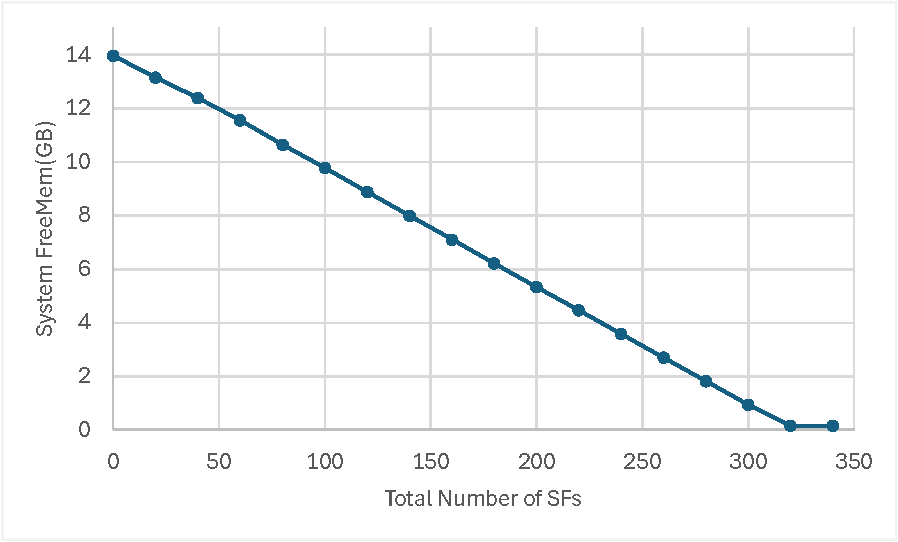
\includegraphics[width=3.2
in]{freemem.pdf}
\caption{The available memory in the system decreases from 14GB to 0.5GB when creating from 0 to 340 SFs and representors on Nvidia BlueField-2 (total 16GB memory).}
\label{fig:arch}
\end{figure}
\fi

\section{Introduction}
Modern network devices support advanced switching and offloading
capabilities, called switchdev mode. In switchdev mode, users can
create multiple virtual ports, or vports, through sysfs and assign
vports to virtual machines or containers. The switchdev mode includes
PFs, the Primary Functions of a PCIe device, with full access to the device's
capabilities. PFs can manage multiple types of vports, including
VFs (Virtual Functions) and SFs (Sub/Scalable Functions).
The switchdev design follows the split model: a fast-path and
slow-path.

As shown in Figure~\ref{fig:arch}, a NIC with advanced offload capability
and flow table rules is
the fast-path, while a corresponding software switch that handles
initial flow rule setup, or the miss traffic processing, is considered the
slow-path. Different vendors such as Nvidia Connect-X or Intel ICE
supports different offload capabilities, but they follow similar
software slow-path design, with OVS or Linux bridge attached with
the slow-path representors, running either on host CPUs or
SmartNIC/DPU ARM cores.

The slow-path ports that handles miss traffic is called representor
netdevs, registered as a regular Linux Ethernet device and is responsible
for administratively configurations of the fast-path vports.
In typical use cases, representor netdev and its representee, vport,
are 1-to-1 mapping: a VF/SF has a its own netdev for fast-path traffic
in host, and another representor netdev for slow-path traffic in DPU.
Such a design is reasonable with tens or hundred-ish vports but when scaling
to thousands of VFs or SFs, the memory resource becomes a limiting factor.
For example, assuming each RX queue has 1024 entries, and each entry
pointing to a 4K-sized page. Assume the netdev has 4 RX queues (controlled
by ethtool -L combined), a netdev will consume 4 * 4K * 1024 = 16MB.
With 1k representor netdevs, the memory consumption can grow
to 16GB (16MB * 1024). We found that majority of memory comes from
the RX memory buffers~\cite{jakub}, i.e., the pre-allocation of
RX queues that handles burst of incoming traffic.

% explain what's rx buffer
The pre-allocation of RX queues and buffers are configured by Linux
ethtool -G/-L option, with different vendors setting different default
value. Nvidia MLX5, by default, pre-allocates 1024 entries in each of
its RX queues, with each entry pointing to a MTU-sized buffer or a page
(without striding RQ). For Intel ICE, its depth RX queue depth is 2045.
A trivial solution is to reduce the number of RX queue entries of
representor netdevs, for example, from 1024/2048 to 64 (the minimum of NAPI
budget). Although this saves memory but a burst of traffic over 64 packets
will be dropped, causing longer connection offload setup time.

The paper describes the current solutions and proposed a new design.
One solution is, instead of having one representor netdev per SF or VF,
redirect all the slow-path traffic from all VFs/SFs to a single netdev,
usually PF or uplink representor. As a result, the PF's RX queue receives
all slow-path traffic from all other representors. In other word, all representors
share the same RX queue memory pool provided by PF. The idea of using PF's
RX qeueu as a shared memory pool is currently used by Intel ICE, Netronome,
Broadcom bnxt, and SFC~\cite{survey}, we called this design "shared RXQ of PF".

%And this saves lots of memory because slow-path traffic is redirected to
%PF, representors no longer needs to create its own RX queues and buffers.
We are able to create 1K SFs and 1K representor netdevs using shared RXQ
of PF. Although this design saves lots of memory, without large and real traffic experiment, it's hard to measure the performance impact of the shared RXQ
of PF design versus no shared design.
In addition, we found that, a VM using a VF/SF can easily monopolize the
entire PF's RXQ, making another VM with VF/SF zero bandwidth.
For example, a VM
running dpdk-testpmd to send 8Mpps of UDP traffic can easily use the
entire PF's RXQ, causing all the rest of VM starvation.

The situation is similar to buffer management problem in shared-memory
packet switches, where the hardware switch has a shared memory buffer pool
for all its output ports and it guarantees both the performance and
fairness~\cite{devlinksb, queuelength} among all output ports.
%The solution couldn't apply to
%our case because it's slow-path traffic, all the hardware traffic
%control or QoS features are not available.
Our proposed solution is inspired by it, but implement it in software.
We describe background in later section, three different designs,
solution to the fairness problem, and finally some performance
number. The paper has the following contributions:
\begin{itemize}
    \item Present the memory consumption requirements for scaling to
          thousands of devices.
    \item Describe the existing solutions from different driver vendors,
          using shared RXQ provided by PF.
    \item Propose a solution to save memory per RX queue by dynamically
          fill and reclaim pages.
    \item Propose a solution using a shared page pool for all netdevs,
          with inherent fairness mechanism.
\end{itemize}
We welcome anyone to review and correct any content in any format (PR, or email to us)\footnote{source: https://github.com/williamtu/netdevconf18-sharedmem}.

\begin{figure}[t!]
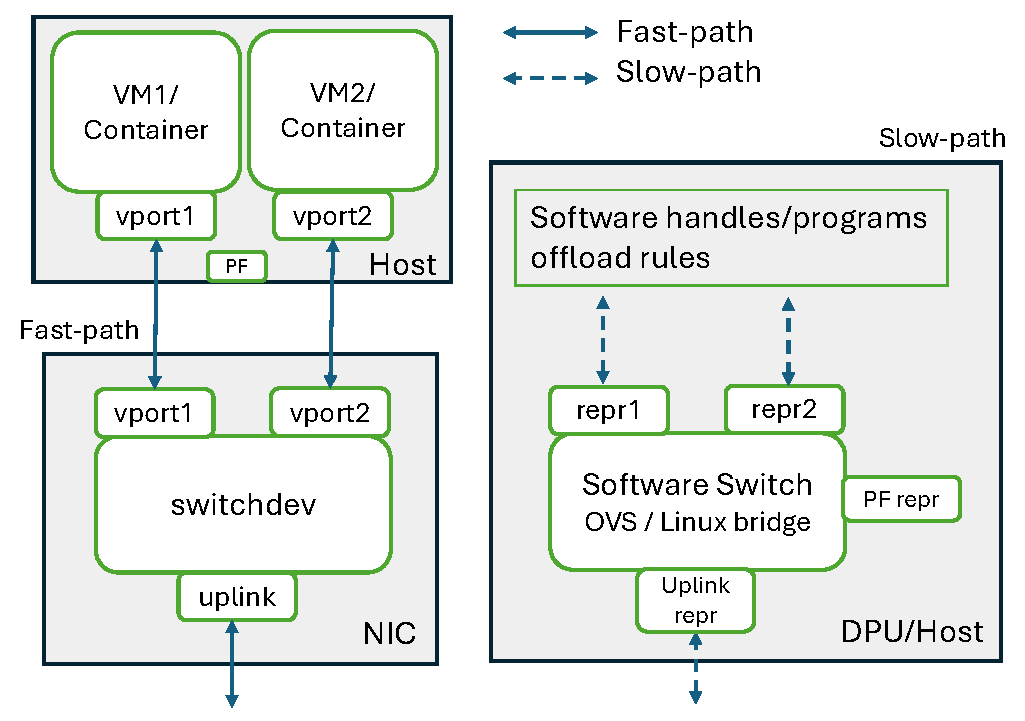
\includegraphics[width=3.2in]{arch.pdf}
\caption{The fast and slow path model. The switchdev in NIC is the fast path handling
hardware offloaded traffic among VFs/SFs, and the DPU which contains representor (repr) netdevs and software switch handles the slow path traffic. The slow-path can be
either in Host, or be part of the NIC.}
\label{fig:arch}
\end{figure}

%This post an important question: how much memory buffer does a representor
%netdev needs to pre-allocate for bursty traffic?
\iffalse
most of these representor netdevs' RX DMA memory
is idle when flows are forwarded directly in hardware to VFs.
In the recent case of smartnic or DPU (data processing unit) such as
Nvidia BlueField and Intel IPU, only the VFs and SFs and a light-weight PF
is exposed to the host side, the PF and representors are created in the
embedded CPU of the smartNIC.
The SmartNIC usually has less memory resources, Nvidia BlueField 3 has
32GB and Intel IPU has NGB, which makes the memory resource more precious.

In this talk we address the memory utilization challenges in DPU, by
first going through all existing solutions in different vendor drivers,
intel, nvidia, broadcom, netronme, and sfc. And we present the shared
memory pool design and implementation.
We should that by sharing the memory 
\fi

\section{Background}
\subsection{Eswitch and Switchdev Mode}
An eSwitch, or embedded switch, is a hardware component within modern network
controllers, such as the Intel Ethernet Controller E810. It is also known as
a Virtual Ethernet Bridge (VEB). The eSwitch is managed by the Physical Function (PF)
driver of the Ethernet or in the case of SmartNIC, managed by the ECPF (Embedded
CPU's PF) that runs in the smartNIC's core. Eswitch can operate in two modes:
Legacy mode and Switchdev mode.

Legacy mode operates based on traditional MAC/VLAN steering rules. Switching
decisions are made based on MAC addresses, VLANs, etc. There is limited ability
to offload switching rules to hardware.
On the other hand, switchdev mode allows for more advanced offloading
capabilities of the E-Switch to hardware. In switchdev mode, more switching
rules and logic can be offloaded to the hardware switch ASIC, for example
push and pop tunneling protocol, connection tracking, etc.
The switchdev mode requires a slow path, software switch such as OVS or
Linux bridge, and representor netdevices that handle miss traffic.
The slow-path handles flows that can not be offloaded or miss the hardware
flow table lookup from the VFs/SFs.
% $$:`Documentation/networking/switchdev.rst <switchdev>` and
%:ref:`Documentation/networking/representors.rst <representors>`.
% devlink dev eswitch show
% devlink dev eswitch set mode switchdev
% need to disable OVS hwoffload
% so it's the iperf TX traffic on VF port that's going to overflow the PF's rxq
\begin{figure}[t!]
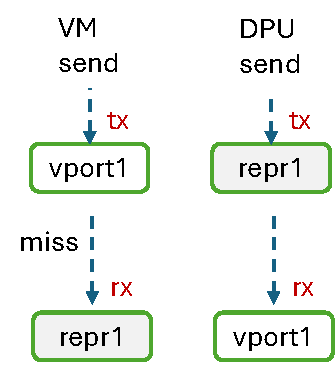
\includegraphics[width=1.5in]{pipe.pdf}
\centering
\caption{The vport (representee) and representor: packets transmitted by the representor 
netdev are delivered to its vport; packets transmitted by the vport are
received by the representor netdev, if it fails to match any offload rule.}
\label{fig:pipe}
\end{figure}

\subsection{Representors}
A vport can be PFs (used by administrator), or VFs or SFs (assigned to VMs
or containers). When the hardware offload table is empty, all packets are 
processed by the slow path. Representor netdev and vport are like a linux
pipe, shown in Figure~\ref{fig:pipe}. Packets transmitted by the representor
netdev from DPU are delivered to its vport; packets transmitted by the vport
from VM are received by the representor netdev, if it fails to match any
offload rule.

% an end-to-end example
For example in Figure~\ref{fig:arch}, VM1 would like to setup a new TCP
connection to VM2. The first TCP SYN packet sent from VM1 misses the
switchdev's flow table, due to no match, and arrives at the receive
queue of vport1's corresponding representor netdev, repr1.
OVS, in this case, with hardware-offload enabled, will parse the protocol
and insert an offload rule, using Linux tc-flower or DPDK rte\_flow interface.
In addition, OVS also forwards/sends the packet to the repr2 port, which
will deliver the packet to vport2's receive queue at VM2.
While VM2 receives the TCP SYN from VM1, VM2 replies with SYN+ACK, and
again goes through the slow path. Once the connection is established
and flow rules are in NIC's flow table, the TCP data stream will be
going through the fast-path in NIC, and OVS in DPU no longer involves
in subsequent packet processing.

Note that the behavior of the slow-path (representor ports and software
switch) should be the same as fast-path (vports and switchdev).
And because representor and vport are acting like pipe, an OpenFlow
rule on a representor netdev applies to a packet on its
receive path is the same as it applies on vport's transmit path.

\iffalse
When the system boots, and before any offload is configured, all packets from
the virtual functions appear in the networking stack of the PF via the
representors.
The PF can configure standard Linux forwarding between representors, the uplink
or any other netdev (routing, bridging, TC classifiers).
Thus, a representor is both a control plane object (representing the function in
administrative commands) and a data plane object (one end of a virtual pipe).
\fi

\subsection{Buffer Pre-allocation for RX Queue}
Network device drivers pre-allocate a circular buffers for absorbing the
burstness of network traffic.
Once packets arrive, NIC can DMA a batch of packets into these pre-allocated buffers,
potentially hundreds of them, before the host CPU is notified/kicked in
by interrupts to process these packets.
For performance reason, NIC contains multiple queues with each queue
represents an NAPI context and an IRQ to kick in to process rx packet.
Usually the number of RX queues is the same as number of CPU that involves
in packet processing.
As shown in Figure~\ref{fig:rxq}, each RX queue contains several entries, 
or queue depth, with each entries
point to a packet buffer. So the amount of pre-allocated memory for RX
is a product of buffer size * number of queues * queue depth.
A typical example of a data center server with 64 cores would be:
4k * 64 queues * 1k entries = 256MB, for a single 64-rxq netdev.

Note that the queue depth, or the number of entries in RX queue, is
not only for tolerating the burstness of traffic, but also the CPU
processing time/jitter of a packet. When CPU is under heavy loading,
a packet arriving RX interrupt might not be able to immediately
kick in the CPU to process packets. Thus a deeper queue depth can
avoid packets being dropped.
In addition, each packet usually has different processing time.
The time for CPU to process a TLS packet is definitely longer than
an ARP packet. Thus, a deeper RX queue also helps avoiding packets
dropped due to intermittently longer packet processing time.

However, memory is not cheap, especially when scaling to 1K devices
and with 1k representor netdevs in DPU. And having several GBs of
pre-allocated memory idle just waiting for a burst of traffic
or even unused when the low traffic volume is a huge resource waste.
We discuss different solutions in later section.

\begin{figure}[t!]
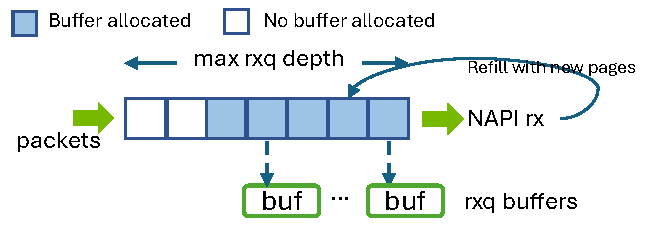
\includegraphics[width=3.0in]{rxq.pdf}
\centering
\caption{Network driver allocates buffers to fill its RX queue. NIC DMA packet
payload into the buffers and NAPI rx function process the packet, refill the 
queue by re-allocating new buffer.}
\label{fig:rxq}
\end{figure}

\section{Design}
% table here shows existing driver's implementation~\cite{buffersize}
With the goal of supporting 1K of SFs/VFs with representor netdevs
on DPU, we set the following requirements: 1) 1k netdevs creation time
around 10 minutes, including configurations and bringing the device up,
2) memory consumption of DPU or host system is within
system limit, and 3) all the VFs/SFs representor get fair share
of receive memory buffer, which leads to fair share of bandwidth.
The following subsections presents four designs: A. Dedicated RXQ,
B. Shared RXQ of PF, C. Adjustable RXQ with shared memory pool, and
D. Shared RXQ with hardware meters.

\subsection{A. Dedicated RXQ}
This design is the default design with minimal or no change.
Dedicated RXQ is used in previous version of Intel ICE before patch~\cite{icepatch}
and also the current version of Marvell Octeontx2~\cite{octeontx2}.
In this design, each representor has its own RXQ, and do not share its
RXQ with any other representors. The design guarantees performance isolation
between representors, but the downsides are that it 1) consumes
lots of RXQ memory in the system, and 2) some NIC hardware has limitation of
how many hardware RX queues it can create. For example, Intel ICE can create up to
1k queues. If users want to use more than 1k representors, there is not
enough queues to assign to each representor netdev.

\subsection{B. Shared RXQ of PF}

\begin{figure}[t!]
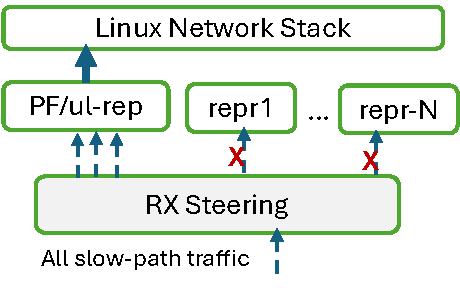
\includegraphics[width=2in]{design1.pdf}
\centering
\caption{Shared RXQ Design: A PF or uplink-representor netdev receives all
slow-path traffic for other representors, and reconstructs their skb
and passes to upper network stacks.}
\label{fig:sharedrxq}
\end{figure}
Since the representor netdev only handles the miss traffic or first
few packets for connection setup, one solution is to aggregate all
slow-path traffic from all representor netdevs into a single one,
usually the PF representor or the uplink representor netdev.
The PF representor acts like an intermediate multiplex layer, and 
it sees all slow path traffic from all other reprensentors.
When packets arrive, it looks up an internal data structure to identify the
original vport id of VF/SF, reconstructs the skb->dev to the correct
orignal netdev, and passes up kernel stack. As a result, the
non-PF or non-uplink representor netdev no longer sees packets
and no need to allocate RX queue, as shown in Figure~\ref{fig:sharedrxq}.

This design saves huge amount of memory because most of the representors'
RX functions are avoided, with all representors' traffic using PF representor
netdev's RXQs. In the case of ICE driver, even the TX
function of the representors are handled by PF representor, making other
representors purely a control/management interfaces.
Different vendors have different implementation, but in general,
the device driver needs to do the following:
%Recall that in Figure~\ref{fig:pipe} the representor and vport are like pipe.
\begin{itemize}
\item RX Hardware Steering: instead of sending slow-path traffic to
each individual representors, the NIC needs to steers/redirects all
slow-path traffic to the PF representor netdev, and mark the packet with
its original vport information, e.g., vport\_id, in metadata or packet buffer.
\item RX in Driver: the PF representor netdev sees all traffic including
others arriving at its RX queues. It needs to keeps a map of vport\_id
to the packet's original netdev struct. By extracting the vport\_id
from metadata, the original netdev is restored to sk\_buff and continue
kernel network stack.
\item TX in Driver: because the vport and representor act like a pipe,
the PF representor netdev need to know which vport's RX queue the packet
should be \emph{send} to. Drivers can use the dst\_entry of skb, or other
per-packet metadata field, and rely on internal switch to deliver the
packet to the vport.
\end{itemize}

\textbf{Pros and Cons:}
Although this design saves lots of memory by redirecting all traffic to
PF representor netdev, users need to tune the following two parameters:
because it consumes only one service
netdev's memory. Depending on number of SF/VFs and traffic volume,
users need to configure two parameters of service netdev:
\begin{itemize}
    \item the number of RXQs should increase to decrease the chance
    of multiple flows from multiple vports rxhash to the same queue,
    e.g., using ethtool -L combined. Most of the drivers limit its max number
    of RXQs to the number of CPUs.
    \item the RX queue depth should increase to absorb more traffic
    burst from multiple vports, e.g., using ethtool -G rx. However, this might
    increase the packet processing latency.
    \item Reduce the NAPI schedule delay, which means NAPI can process
    packets as soon as possible when packets arrived. This lowers the chance
    of RXQ utilization grows to fast or overflow. (I don't know any tool to do this).
\end{itemize}

The design is simple to implement, but we found that it suffers from
a \emph{fairness} issue. A single high volume sender, ex: dpdk-pktgen,
sending to its vport and with packets arriving at slow path, can easily
consume all the buffers in the PF representor netdev's RXQ.
And because all other representors share the same PF's RXQ, this makes
other representor and its vport traffic being dropped due to no
available RX buffer at all. An example setup script to show case the issue
using OVS is provided in Listing~\ref{lst:fairness}.

\subsection{C-1. Adjustable RXQ Depth}
If the shared RXQ of PF suffers from fairness issue, another solution is to
{\em not} sharing the RXQ, but think about other ways to save memory.
For every RXQ in every netdev, existing network drivers implement \emph{static}
RXQ allocation.  Whenever a driver initializes, it always pre-allocates the number
of buffers to the full RXQ depth, and whenever a batch of packets arrived and
processed by NAPI poll, device driver again refills to full by re-allocating
buffers to the \emph{full} RXQ depth.

To save memory, instead, the adjustable RXQ depth does not refill to full
RXQ depth, but only to a threshold value, called low\_watermark.
For example, the mlx5 driver, by default, always tries to allocate to
full 1024 rxq buffers. With adjustable RXQ, the following logic is applied
when a driver is receiving packets in its NAPI context:
\begin{itemize}
    \item NAPI busy: allocate buffers and refill to full queue depth, high\_watermark.
    The high\_watermark equals the max RXQ depth set by ethtool -G rx.
    \item NAPI interrupt: allocate buffers and refill to low watermark if
    current RXQ depth is lower than low watermark
    \item NAPI interrupt: do not allocate and do not refill if current
    RXQ depth is higher than low\_watermark.
\end{itemize}

\textbf{Pros and Cons: }
We set the low\_watermark to be 128 (2 * NAPI\_BUDGET). 
The low\_watermark means the minimal available RXQ buffers to handle the
worst case of traffic burst. At driver initialization time, all queues
are allocated only up-to the low\_watermark. Once the first burst
of traffic arrives, users might see more packets dropped compared
to full rxq depth allocation (1024). Fortunately, a NAPI busy state will
trigger driver to refill RXQ to its full depth, making the performance
impact minimal. In this design, we pay the performance price to save
memory. The first burst traffic of a connection definitely see more
packets dropped, and once in NAPI-busy, the driver acts the same as
static RX queue allocation.

%The high\_watermark is the max RX queue depth, which is the same value
%set in static allocation, the rxq depth set by (ethtool -G rx)
Such a design saves memory at driver initialization, as well as when at
the NAPI-interrupt state, device driver will slowly return RXQ buffers back
to kernel due to packet arrives but driver does not re-allocate.
However, what if an RXQ is in NAPI-interrupt state, but there is no packet
arrived to trigger returning buffers to system? Then driver needs to detect
and drain the RX queue back to the low\_watermark.

We implement this prototype and evaluate its impact in performance evaluation section.

\begin{figure}[t!]
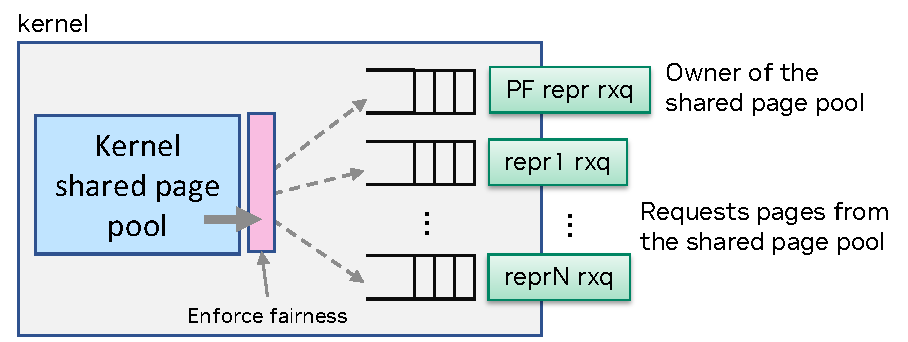
\includegraphics[width=3.2in]{shared_page_pool.pdf}
\centering
\caption{The adjustable RXQ from multiple reprs requests pages from the shared page pool.
A fairness layer guarantees each repr gets the proportional shares of the total available memory.}
\label{fig:shared_page_pool}
\end{figure}

\subsection{C-2. Adjustable RXQ Depth with Shared Page Pool}
% TODO: limitation, single NIC DMA device, or how about virtual devices such as multiple veth?
We found that the memory savings with the design of adjustable RXQ depth
might not be enough.
Currently each RXQ creates its own kernel page pool, and in NAPI, refilling
the RXQ buffers by allocating a page pool entry from its own per-queue page pool.
When scaling to thousands of representor netdevs, there is no guarantee that
all the representor netdev gets fair shares of system memory. That is, the later
created representor netdevs might see system out-of-memory for initializing its RXQ,
even with the Adjustable RXQ Depth design.

We propose shared page pool, a layer of page pool that runs on top of current
Linux page pool APIs. The shared page pool supports for a group of netdevs
to register as user, request buffers to use in its RXQs, and the shared memory
pool fairly allocate memory for each user based on the its current usage and
total available memory in the pool.

Figure~\ref{fig:shared_page_pool} shows the idea.
Assume N representor netdevs, with each has one RXQ. In the beginning,
a special netdev, PF or uplink representor, creates the shared page pool,
and joins itself into the pool. The rest of netdevs created later join the shared page pool,
by registering itself to the pool, and requests RXQ buffers by calling
the alloc and free API to get or put the page into shared pool.
%We assume \emph{no lock} is required,
%by creating the shared page pool per-CPU NAPI context, which NAPI scheduler
%will guarantee not scheduling two NAPIs poll sharing the same pool on
%different cores.
We define the following APIs:
\begin{verbatim}
# Creates page pool, return the handler
spp = shared_pp_create(
    max_num_devs, page_pool_size, …);

# Return a user id for registerd user
spp_uid1 = shared_pp_join(spp, rep1,
    qid, threshold);
spp_uid2 = shared_pp_join(spp, rep2,
    qid, threshold);
    
# Representor NAPI processes packets and
# refills, and bounded by max_usage, return
# -ENOMEM if overflow
shared_pp_dev_alloc_page(spp, spp_uid1);
shared_pp_dev_alloc_page(spp, spp_uid2);
shared_pp_put_page(spp, spp_uid1);

#Leave the share page pool
shared_pp_leave(spp, spp_uid1); 
\end{verbatim}

But how to solve the fairness issue?
The problem of multiple RXQs sharing a single page pool is
very similar to the shared memory for multiple ports problem in
hardware switch~\cite{queuelength}, configured using devlink-sb~\cite{devlinksb}.
Instead of hardware switch memory, here we have shared page pool memory,
and in contract to switch output ports competing for shared buffers,
here it's the RXQs from different representor netdevs.
Given the similarity, we re-use the dynamic threshold formula to define
the max number of RXQ buffers assigned for each RXQ. That is,
the max\_usage of a particular shared page pool user is
defined by a to\_alpha value below:

\begin{equation}
\alpha = 2^{(\text{to\_alpha} - 10)}
\end{equation}
and the to\_alpha is ranged between 0 to 20, and with $\alpha$, we can get
max\_usage below:
\begin{equation}
\text{max\_usage} = \frac{\alpha}{1 + \alpha} \times \text{Free\_Buffer}
\end{equation}

Note that the Free\_Buffer means the currently available free pages
in the shared page pool. As a result, each user of the pool have a
dynamic max\_usage based on currently page pool memory utilization.

For example, assuming to\_alpha value is 11, so $\alpha = 2$, $ \text{max\_usage}
= 1/2 * \text{Free\_buffer} $.
This mean at any given point of time, a representor netdev can use up to half of
the shared memory pool, even if there is no other users. An as more and more
users join the shared page pool, the Free\_buffer decreases, but with each driver
frees up memory after processing packets, the Free\_buffer will increase again.

\textbf{Pros and Cons:} The design is simple but leaves the user to configure
the value of $\alpha$. When the traffic distribution to different representors
is uneven, a large $\alpha$ will limit the high volume representor to use all
the available memory, while a smaller $\alpha$ value with a even traffic distribution
might still cause unfairness or some representors get no page.
The paper~\cite{queuelength} is based on simulation, and we don't have a good
tool or benchmark traffic pattern to measure the effectiveness of the design.

Note that existing Linux page pool requires registering a DMA device to do
dma map and unmap, and because representors all share the same DMA device,
so they can share single page pool. Other use cases are non-physical device
such as Linux veth/tun/tap.

\subsection{D. Shared RXQ with Hardware meters}
\begin{figure}[t!]
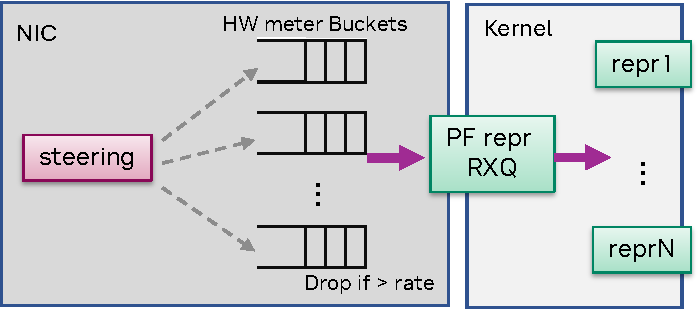
\includegraphics[width=3in]{meter.pdf}
\centering
\caption{The design uses hardware meter in steering to rate-limit each repr's traffic,
so the RXQ buffers won't be monopolized by a particular vport/repr.}
\label{fig:shared_page_pool}
\end{figure}

Another approach to solve the fairness and memory issue is to seek for hardware
support. This design is based on A. Shared RXQ of PF, and enforces the fairness
\emph{before} packets arriving the RXQ buffer.
Most of the NICs supports hardware metering, which allows users to configure it
as a rate limiter, either in PPS (packets-per-second) or BPS (bytes-per-seconds).
Before traffic arrives and consumes the RXQ's buffer, the meter rate limiter
might pass the packet to continue using the shared RXQ of PF, or, the meter
rate limiter might drop the packet if a particular flow of a vport is over
its rate.

\textbf{Pros and Cons:} We implemented this design and realize a couple issues.
First, not all NIC hardware support meters. The implementation is vendor-specific
and comes with different limitations. Second, setting the right meter rate is hard.
Users usually have no prior knowledge
about how fast the DPU/CPU can process the slow path traffic, either in terms of
PPS or BPS. Setting tool low under utilizes the RXQs and setting rate too high
causes fairness issue.
Finally, maintaining thousands of steering rules with meters is not easy, as the
steering rules might collide with other rules with different priorities.

\begin{table}[h!]
\centering
\footnotesize
\begin{tabular}{|l|p{3.6cm}|} \hline
\textbf{Driver} &  \textbf{Implementation}\\ \hline \hline
Nvidia MLX5 & Shared RXQ of PF and \newline Adjustable RXQ \\ \hline
Intel ICE & Shared RXQ of PF~\cite{icepatch} \\ \hline
Broadcom BNXT & Shared RXQ of PF ~\cite{survey} \\ \hline
Netronome NFP & Shared RXQ of PF~\cite{survey} \\ \hline
Solarflare SFC & Shared RXQ of PF~\cite{survey} \\ \hline
Marvell Octeontx2 & Dedicated repr netdevs~\cite{octeontx2} \\ \hline
\end{tabular}
\caption{Summary of existing network drivers and its representor solution.}
\label{tab:vendors}
\end{table}

\section{Implementation}
Most of the network device drivers with representor chooses the shared
RX Queue design, which saves memory at the price of possible
fairness limitation. Table~\ref{tab:vendors} show a summary of 

\subsection{New Devlink Eswitch Attribte: spool}
Given the fairness issue, we'd like to propose a new devlink eswitch attribute
for users to enable or disable the Shared RXQ of PF.
When memory is a precious resources such as SmartNIC or DPU, enabling the Shared RXQ
saves the most memory as it only uses the RXQ from the PF. And the memory consumption
does not grow linearly as the number of representors grows.
On the other hand, if users worry about potencial fairness issue or malicious users,
then disabling shared RXQ and fallback to the dedicated RXQ can solve the problem.
Below is the proposed devlink UAPI example~\cite{spool}:

The attribute supports only in switchdev mode.
\begin{verbatim}
$ devlink dev eswitch set pci/0000:08:00.0 \
   mode switchdev spool enable
$ devlink dev eswitch show pci/0000:08:00.0
   pci/0000:08:00.0: mode legacy \
   inline-mode none encap-mode basic \
   spool enable
$ devlink dev eswitch set pci/0000:08:00.0 \
   mode switchdev spool disable
\end{verbatim}

With this, existing drivers will need to consider supporting both
modes, shared RXQ mode or dedicated mode. (Or return -ENOSUPP).

\section{Performance Evaluation}

We conduct our experiment with two servers connected back-to-back using
two x86 host, shown in Figure~\ref{fig:testbed}.
Each host is equipped with one dual port BlueField-2 card.
Each x86 host consists of 10 cores and 32GB of RAM. The BlueField-2
is an 8-cores Cortex-A72, with 16GB of RAM. BlueField, by default, runs OVS kernel
datapath with hardware-offload enabled.

\subsection{Memory Consumption}
Linux kernel today provides several memory profiling tool, such as /proc/meminfo,
/proc/slabinfo. However, there is no tool to measure how much memory is consumed
by a particular network device driver, or a netdev. We start by creating 200 SF representors,
and measure the difference of the total system free mem, MemFree field in /proc/meminfo.
The SF creation and setup is done by the script in Listing~\ref{lst:sf}.

Table~\ref{tab:memory} shows the memory consumption of each SF-repr and its breakdown.
We conclude that, by default RXQ depth of 1024, one SF-repr takes 2.86MB of kernel
memory, and among the 2.86MB, 1.83 is consumed by page pool for the RXQ buffers,
around 0.11MB is consumed by firmware, and the rest of 0.9MB is for others
such as slab, ex: kmalloc, kzalloc, and other kernel netdev structures.
When increase from 1 RXQ to 2 RXQs, the memory consumption also increases linearly, as expected.
\begin{figure}[t!]
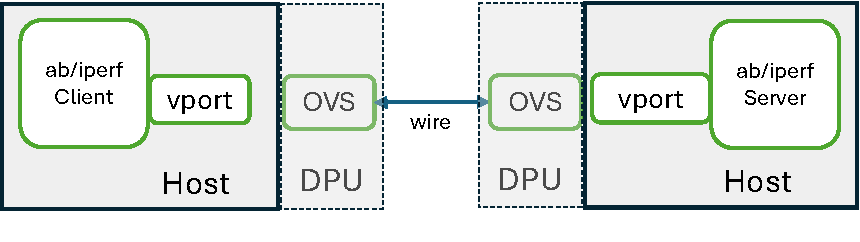
\includegraphics[width=3.2in]{testbed.pdf}
\centering
\caption{Back-to-back setup with x86 host and ARM DPU for performance evaluation.}
\label{fig:testbed}
\end{figure}

\begin{table}[h!]
\centering
\footnotesize

\begin{tabular}{|c|c|c|c|c|}
\hline
\textbf{} & \textbf{1RXQ total} & \textbf{Page Pool} & \textbf{FW} & \textbf{2RXQ} \\ \hline \hline
\textbf{128}  & 1.1   & 0.2  & 0.113 & 2.835 \\ \hline
\textbf{256}  & 1.3   & 0.4  & 0.114 & 2.915 \\ \hline
\textbf{512}  & 1.805 & 0.78 & 0.114 & 2.99  \\ \hline
\textbf{1024} & 2.86  & 1.83 & 0.114 & 5.025 \\ \hline
\textbf{2048} & 4.935 & 3.93 & 0.115 & 9.25  \\ \hline
\end{tabular}
\caption{Memory consumption of a SF-repr and its breakdown of page pool and Firmware usage.}
\label{tab:memory}
\end{table}

\subsection{Static Queue Size}
Before enabling the dynamic adjustable RXQ size, we first analyze the performance impact
of statically configure different RXQ size, from queue depth of 64 to 2048.
We ran Apache ab benchmark~\cite{ab}, with client on one of the x86 host and
server on another x86 host. We disable OVS hardware-offload in DPU so that all traffic
can flow through the representor netdev. We than statically adjust the representor
netdev's RXQ depth using ethtool -G. 

Table~\ref{tab:ab1} shows the result of Apache ab benchmark sending 1 million requests
with concurrency level of 100. We report the following metrics:
\begin{itemize}
    \item Time to complete (sec): total time taken for completing the 1 million requests.
    \item out\ of\ buffers (K): a firmware counter, rx\_out\_of\_buffer, reporting number of packets dropped due to no RXQ buffer available.
    \item Requests (K) / sec: average HTTP requests per seconds
    \item Connection Time (ms) and SD: average connection time, including connect, processing, and waiting, of the 1 million connections and their standard deviation (SD).
\end{itemize}
We found although larger queue depth, 1024 or 2048, consumes more memory, but they
performance comparatively well, as they shows shorter time to complete, less packets
being dropped, and lower jittering (SD is smaller).

\begin{table}[h!]
\centering
\footnotesize
\begin{tabular}{|p{0.6cm}|p{1.2cm}|p{1.2cm}|p{1.2cm}|p{0.8cm}|p{1cm}|} \hline
\textbf{} & \textbf{Time to complete (sec)} & \textbf{out of buffers (K)} & \textbf{Requests / sec (K)} & \textbf{Conn Time (ms)} & \textbf{Conn Time SD} \\ \hline \hline
\textbf{64}   & 45.6  & 104   & 21.9 & 5 & 32  \\ \hline
\textbf{128}  & 29.48 & 71    & 33.9 & 3 & 20  \\ \hline \hline
\textbf{256}  & 24.55 & 5.89  & 40.7 & 2 & 4   \\ \hline
\textbf{512}  & 24.06 & 1.2   & 41.5 & 2 & 2.2 \\ \hline
\textbf{1024} & 24.09 & 0     & 41.5 & 2 & 1.9 \\ \hline
\textbf{2048} & 24.03 & 0     & 41.2 & 2 & 1   \\ \hline
\end{tabular}
\caption{Result of Apache ab benchmark with 1 million requests and 100 concurrent connections.}
\label{tab:ab1}
\end{table}


\subsection{Dynamic Queue Size}
We implement the idea of adjustable queue side, by setting the low\_watermark to
be queue depth of 128, and high water\_mark is configured between 256 to 2048, using
ethtool -G. The mlx5 driver initializes its RXQ only to the low\_watermark.
When the mlx5 napi poll function detects in busy state, it refills the
RXQ to its high watermark. Otherwise if napi poll is in interrupt state, the driver
doesn't refill at all if the current available buffers in the RXQ is higher than
the low\_watermark. In interrupt mode, we only refill when available buffers in the RXQ
is lower than the low\_watermark.

Table~\ref{tab:ab2} shows the results.
\begin{table}[h!]
\centering
\footnotesize
\begin{tabular}{|p{0.6cm}|p{1.2cm}|p{1.2cm}|p{1.2cm}|p{0.8cm}|p{1cm}|} \hline
\textbf{} & \textbf{Time to complete (sec)} & \textbf{out of buffers (K)} & \textbf{Requests / sec (K)} & \textbf{Conn Time (ms)} & \textbf{Conn Time SD} \\ \hline \hline
\textbf{256}  & 24.6  & 22   & 40.1 & 2 & 9.6 \\ \hline
\textbf{512}  & 24.1  & 2.1  & 41.3 & 2 & 2.9 \\ \hline
\textbf{1024} & 24.2  & 65   & 41.2 & 2 & 2   \\ \hline
\textbf{2048} & 23.9  & 95   & 41.7 & 2 & 1.8 \\ \hline
\end{tabular}
\caption{Result of Apache ab benchmark with 1 million requests and 100 concurrent connections.}
\label{tab:ab2}
\end{table}

Compared Table~\ref{tab:ab2} with Table~\ref{tab:ab1}, the dynamic queue size shows noticeable
performance difference. We first observe that even with queue depth high\_watermark set to 2048,
we still see several packets drop. This is due to the driver initializes only at low\_watermark,
so the first burst of traffic definitely triggers out of buffer drops.
In addition, although the total time to complete and the average connection time are almost the
same, the jittering (SD) is much higher due to more packets being dropped and retransmission.


Finally, we compare 20 seconds tcp single connection performance using iperf3 in Table~\ref{tab:iperf}. 
The dynamic queue size design performs almost the same, with the worst case of
dropping around 8\% when queue size is 2048.
Note that all the experiments are done by disabling the hardware offload.
When enabling hardware offload, most of the traffic are processed in hardware and
we're not able to see any performance difference.
In conclusion, we feel that the performance impact will be even smaller in production
environment when hardware offload is always enabled.

\begin{table}[h!]
\centering
\footnotesize
\begin{tabular}{|l|c|c|}
\hline
%\textbf{} & \multicolumn{2}{|c|}{\textbf{Test Time: 20s}} \\ \hline
\textbf{} & \textbf{BW Gbps (Static)} & \textbf{BW Gbps (Dynamic)} \\ \hline
\textbf{64}   & 3.78 & 2.71 \\ \hline
\textbf{128}  & 5.23 & 5.19 \\ \hline
\textbf{256}  & 6.03 & 6.15 \\ \hline
\textbf{512}  & 6.25 & 6.40  \\ \hline
\textbf{1024} & 6.08 & 5.79 \\ \hline
\textbf{2048} & 6.03 & 5.49 \\ \hline
\end{tabular}
\caption{TCP bandwidth comparison of static queue size v.s dynamic queue size, with HW offload disabled.}
\label{tab:iperf}
\end{table}



\section{Conclusion}
Scaling to thousands of netdevs is challenging.



%numbers.\footnote{This is how your footnotes should appear.} Separate them from the text by a short horizontal line. 
\section{Acknowledgments}
We'd live to thank many people for their valuable feedbacks, from internally and the community.

% discussion
% NAPI budget, net_dim, API
% why hardware and software TC QOS doesn't work

For technical questions about Microsoft Word formatting please seek online tutorials. For other questions about your manuscript please contact: {\tt ISEA2015-info@sfu.ca}

\bibliographystyle{isea}
\bibliography{isea}
\section{OVS Script} \label{sec:bash_script}
\begin{lstlisting}[language=sh, caption={Bash Script for Database Backup}, label={lst:bash_script}]
#!/bin/bash

# similar setup for Linux bridge, but disable HW offload by setting aging=0
PF1=eth2
VFREP1=eth4
VFREP2=eth5
VF1=eth6
VF2=eth7
NS1=ns1
NS2=ns2
NS3=ns3
NS4=ns4
SF1=enp8s0f0s88
SF2=enp8s0f0s99
SFREP1=en8f0pf0sf88
SFREP2=en8f0pf0sf99

setup_dev_ns()
{
        ns=$1
        vfdev=$2
        ip=$3

        ip netns del $ns || true
        ip netns add $ns
        ip link set dev $vfdev netns $ns
        ip netns exec $ns ifconfig $vfdev ${ip}/24 up
        ip netns exec $ns iperf3 -s  -u -D
        ip netns exec $ns iperf3 -s -D
        ip netns exec $ns netserver
}

test_dpdk()
{
        ip netns exec $NS1 bash
# don't use "--txonly-multi-flow"
echo 1280 > /sys/devices/system/node/node0/hugepages/hugepages-2048kB/nr_hugepages
dpdk-testpmd -l 0-3 --socket-mem=512  -a 0000:08:00.2 -- -i --nb-cores=1 --forward-mode=txonly \
--eth-peer=0,b8:3f:d2:ba:65:9e --txpkts=64 --txq=1 --rxq=1 --stats-period=1 --txonly-multi-flow \
--total-num-mbufs=2048
        exit

}

setup_ovs()
{
        /usr/share/openvswitch/scripts/ovs-ctl stop
        rm -f /etc/openvswitch/conf.db

        echo 2 > /sys/class/net/$PF1/device/sriov_numvfs
        python2 /usr/bin/mlx_fs_dump -d 0000:08:00.0 > /root/net-next/fdb.txt
        /usr/share/openvswitch/scripts/ovs-ctl start
        ovs-vsctl set Open_vSwitch . other_config:hw-offload=false 
        # need to restart OVS
        ovs-vsctl add-br ovsbr0
        ovs-vsctl add-port ovsbr0 $PF1
        ovs-vsctl add-port ovsbr0 $VFREP1
        ovs-vsctl add-port ovsbr0 $VFREP2
        #ethtool -L $PF1 combined 2 # mlx5e_napi_poll busy=true
        echo "bring up device" > /dev/kmsg
        ip link set dev $PF1 up

        #ethtool -L $VFREP1 combined 2
        ip link set dev $VFREP1 up
        ip link set dev $VFREP2 up

        setup_dev_ns $NS1 $VF1 192.167.111.1
        setup_dev_ns $NS2 $VF2 192.167.111.2

        ip netns exec $NS1 arp -s 192.167.111.2 d2:a0:5f:ad:a4:e4
        ip netns exec $NS1 ip link set dev eth6 addr 66:0f:91:31:0a:89
        ip netns exec $NS2 arp -s 192.167.111.1 66:0f:91:31:0a:89
        ip netns exec $NS2 ip link set dev eth7 addr d2:a0:5f:ad:a4:e4
        #ip netns exec $NS1 iperf -c 192.167.111.2 -t5 -i1
        ip netns exec $NS1 ping -i .05 -c10 192.167.111.2
        ip netns exec $NS2 ping -i .05 -c10 192.167.111.1
        ip netns exec $NS1 iperf3 -u -b10G -c 192.167.111.2 -t1 -i1
        ip netns exec $NS1 iperf3 -c 192.167.111.2 -t2 -i1
}

devlink dev eswitch set pci/0000:08:00.0 mode switchdev
setup_ovs
\end{lstlisting}

\end{document}
%challenges and takeaways
%\begin{figure}[h]
%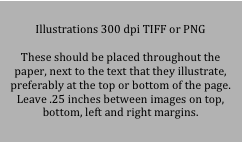
\includegraphics[width=3.31in]{figure.png}
%\caption{This is an example of figure caption. Note that all figures, and tables are to be referenced in the text. \copyright Respect Copyright.}
%\end{figure}
